% chapters/03-success-stories.tex

\chapter{Success Stories and Lessons Learned}\label{ch:success-stories-and-lessons-learned}

\begin{importantbox}
This chapter brings theory to life through real-world success stories.\ Each narrative highlights how entrepreneurs navigated specific challenges in the Nigerian market, offering practical insights you can apply to your own journey.
\end{importantbox}

\section{UK Case Study: Sarah's FinTech Market Entry Success}\label{sec:uk-case-study:-sarah's-fintech-market-entry-success}

Let's start with Sarah's use-case.\ As she described her plans to enter the Nigerian market, there's the familiar mix of excitement and apprehension in her eyes.\ ``Nigeria's fintech space seems incredibly dynamic,'' she said, stirring her coffee, ``but how do you even begin to build trust with potential customers?''

\subsection{The Journey: From The Trading Desk to Lagos Fintech Pioneer}\label{subsec:the-journey:-from-the-trading-desk-to-lagos-fintech-pioneer}
\begin{tcolorbox}[colback=white,colframe=primarydark,title=\textbf{Sarah's Profile}]
\begin{itemize}
    \item \textbf{Background:} 15 years in investment banking
    \item \textbf{Previous Role:} Head of Trading, Major Bank
    \item \textbf{Market Entry:} Cross-border payments solution
    \item \textbf{Initial Capital:} £55,000
    \item \textbf{Time to Market:} 9 months
\end{itemize}
\end{tcolorbox}

Sarah's approach to market penetration was methodical yet innovative.\ She developed what I now call the ``Trust Triangle'' strategy:

\begin{figure}[h]
    \centering
    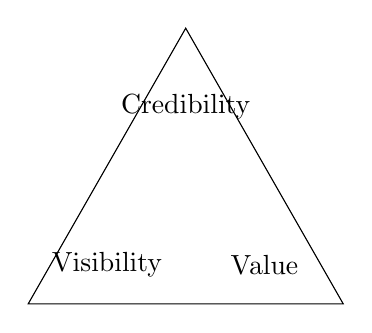
\begin{tikzpicture}
        % Trust Triangle visualization
        \draw (0,0) -- (4,0) -- (2,3.5) -- cycle;
        \node at (2,2.5) {Credibility};
        \node at (1,0.5) {Visibility};
        \node at (3,0.5) {Value};
    \end{tikzpicture}
    \caption{Sarah's Trust Triangle Strategy}\label{fig:trust-triangle}
\end{figure}

\subsection{Key Success Factors}\label{subsec:key-success-factors}
\begin{enumerate}
    \item \textbf{Strategic Partnership Selection}
    Sarah didn't just seek partnerships; she created what she called ``trust bridges.'' ``Each partner,'' she explained later, ``wasn't just a business relationship but a credibility ambassador.''

    \item \textbf{Localized Product Development}
    Instead of simply transplanting her London solution, she spent months adapting it to local needs.``The Nigerian market taught me that efficiency without cultural relevance is just sophisticated failure,'' she said.

    \item \textbf{Phased Market Entry}
    She used what I now call the ``Concentric Circle Approach'':
    \begin{itemize}
        \item Phase 1: Corporate clients (established trust)
        \item Phase 2: SME network (built volume)
        \item Phase 3: Retail customers (achieved scale)
    \end{itemize}
\end{enumerate}

\section{US Case Study: Mike's E-commerce Evolution}\label{sec:us-case-study:-mike's-e-commerce-evolution}

Mike started with a ``bulletproof'' plan for Nigerian e-commerce.\ After a short review, that plan was in pieces – he realised something much better.

\subsection{The Comprehensive Journey}\label{subsec:the-comprehensive-journey}
\begin{tcolorbox}[colback=white,colframe=primarydark,title=\textbf{Mike's Challenge Areas}]
\begin{enumerate}
    \item \textbf{Technology Adaptation}
    \begin{itemize}
        \item Initial Challenge: Platform optimized for high-speed internet
        \item Solution: Progressive Web App with offline capabilities
        \item Result: 300\% increase in successful transactions
    \end{itemize}

    \item \textbf{Last-Mile Delivery}
    \begin{itemize}
        \item Initial Challenge: Traditional delivery models failing
        \item Solution: Hybrid network of official and local partners
        \item Result: Delivery success rate from 65\% to 84\%
    \end{itemize}

    \item \textbf{Payment Integration}
    \begin{itemize}
        \item Initial Challenge: High payment failure rates
        \item Solution: Multi-provider payment orchestration
        \item Result: Payment success rate increased to 94\%
    \end{itemize}

    \item \textbf{Customer Acquisition}
    \begin{itemize}
        \item Initial Challenge: High CAC through traditional channels
        \item Solution: Community-based marketing approach
        \item Result: CAC reduced by 60\%
    \end{itemize}
\end{enumerate}
\end{tcolorbox}

\subsection{Technology Adaptation Deep Dive}\label{subsec:technology-adaptation-deep-dive}
Mike's journey with technology adaptation offers particularly valuable lessons.
Here's how he transformed his approach:

\begin{center}
\begin{tabularx}{\textwidth}{>{\raggedright\arraybackslash}X >{\centering\arraybackslash}X >{\raggedright\arraybackslash}X}
    \toprule
    \textbf{Feature} & \textbf{Before} & \textbf{After} \\
    \midrule
    Page Load & 12 seconds & 3 seconds \\
    Offline Access & None & Full catalog browsing \\
    Image Loading & Standard & Progressive \\
    Data Usage & 4MB per session & 800KB per session \\
    \bottomrule
\end{tabularx}
\end{center}

\subsection{Last-Mile Innovation}\label{subsec:last-mile-innovation}
Mike's solution to the delivery challenge became what I call the ``Hub and Spoke Plus'' model:

\begin{figure}[h]
    \centering
    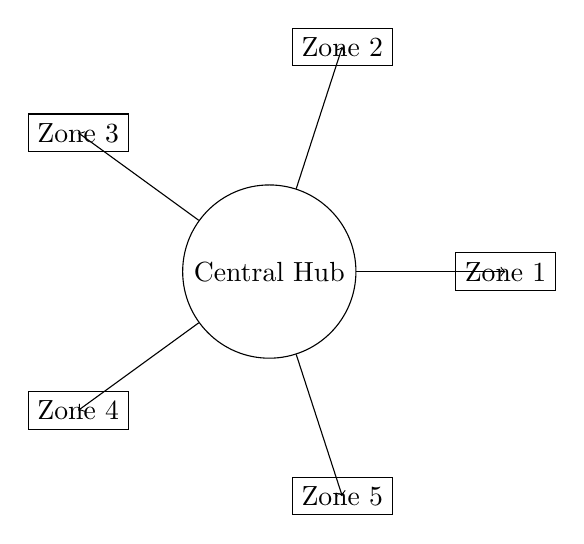
\begin{tikzpicture}
        % Delivery network visualization
        \node[draw, circle] (hub) at (0,0) {Central Hub};
        \foreach \angle/\label in {0/Zone 1,72/Zone 2,144/Zone 3,216/Zone 4,288/Zone 5}
        {
            \node[draw] at (\angle:3) {\label};
            \draw[->] (hub) -- (\angle:3);
        }
    \end{tikzpicture}
    \caption{Hub and Spoke Plus Delivery Model}
\end{figure}

\section{UAE Case Study: Ahmed's Partnership Mastery}\label{sec:uae-case-study:-ahmed's-partnership-mastery}

Ahmed's story is particularly interesting because it shows how traditional trading expertise can be enhanced through strategic local partnerships.\ ``In Dubai,'' he said during a strategy sessions, ``relationships matter.\ But in Nigeria, they're everything.''

\subsection{Partnership Development Framework}\label{subsec:partnership-development-framework}
\begin{tcolorbox}[colback=white,colframe=primary,title=\textbf{Ahmed's Partnership Matrix}]
\begin{enumerate}
    \item \textbf{Identification Phase}
    \begin{itemize}
        \item Market segment mapping
        \item Capability gap analysis
        \item Cultural alignment assessment
    \end{itemize}

    \item \textbf{Engagement Strategy}
    \begin{itemize}
        \item Phased commitment approach
        \item Value proposition clarity
        \item Risk-sharing framework
    \end{itemize}

    \item \textbf{Relationship Management}
    \begin{itemize}
        \item Regular value assessment
        \item Conflict resolution protocol
        \item Growth planning integration
    \end{itemize}
\end{enumerate}
\end{tcolorbox}

\section{Canadian Case Study: Lisa's AgriTech Revolution}\label{sec:canadian-case-study:-lisa's-agritech-revolution}

Lisa's journey is a masterclass in combining sustainability with scalability.\ When she shared her entry plans, this stuck with me: ``I'm not just building a business; I'm building an ecosystem.''

\subsection{Distribution Network Development}
\begin{figure}[h]
    \centering
    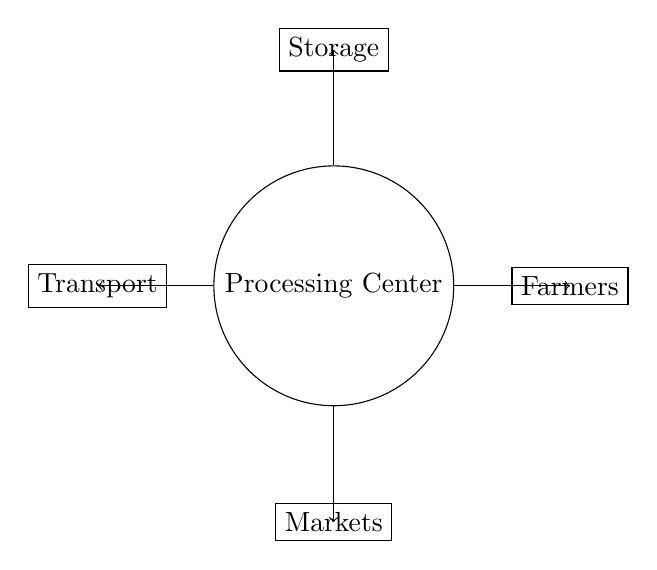
\begin{tikzpicture}
        % Agricultural network visualization
        \node[draw, circle] (hub) at (0,0) {Processing Center};
        \foreach \angle/\label in {0/Farmers,90/Storage,180/Transport,270/Markets}
        {
            \node[draw] at (\angle:3) {\label};
            \draw[->] (hub) -- (\angle:3);
        }
    \end{tikzpicture}
    \caption{Integrated Agricultural Distribution Network}
\end{figure}

\subsection{Sustainable Practices Integration}\label{subsec:sustainable-practices-integration}
\begin{tcolorbox}[colback=white,colframe=primary,title=\textbf{Sustainability Framework}]
\begin{enumerate}
    \item \textbf{Environmental Impact}
    \begin{itemize}
        \item Solar-powered storage facilities
        \item Water conservation systems
        \item Waste reduction protocols
    \end{itemize}

    \item \textbf{Economic Sustainability}
    \begin{itemize}
        \item Farmer financing programs
        \item Market price stabilization
        \item Value-added processing
    \end{itemize}

    \item \textbf{Social Responsibility}
    \begin{itemize}
        \item Community training programs
        \item Women farmer initiatives
        \item Youth engagement projects
    \end{itemize}
\end{enumerate}
\end{tcolorbox}

\section{Key Lessons Learned}\label{sec:key-lessons-learned}

Looking across these success stories, several universal principles emerge:

\begin{tcolorbox}[colback=white,colframe=primarydark,title=\textbf{Universal Success Principles}]
\begin{enumerate}
    \item \textbf{Adaptive Innovation}
    Success comes not from transplanting foreign solutions, but from thoughtful adaptation to local conditions.

    \item \textbf{Partnership Primacy}
    The quality of your local partnerships often determines the speed and scale of your success.

    \item \textbf{Cultural Integration}
    Understanding and embracing local business culture is not optional – it's fundamental to success.

    \item \textbf{Phased Growth}
    The most sustainable successes come from methodical, phased approaches rather than big-bang launches.
\end{enumerate}
\end{tcolorbox}

\begin{workshopbox}
\textbf{Chapter Application Exercise}

1. Success Pattern Analysis
\begin{itemize}
    \item Identify three success patterns most relevant to your business: \_\_\_\_\_\_\_\_\_
    \item List specific ways to apply each pattern: \_\_\_\_\_\_\_\_\_
    \item Potential challenges in implementation: \_\_\_\_\_\_\_\_\_
\end{itemize}

2. Risk Mitigation Planning
\begin{itemize}
    \item Key risks identified from case studies: \_\_\_\_\_\_\_\_\_
    \item Relevant mitigation strategies: \_\_\_\_\_\_\_\_\_
    \item Required resources or partnerships: \_\_\_\_\_\_\_\_\_
\end{itemize}

3. Action Planning
\begin{itemize}
    \item Immediate action items: \_\_\_\_\_\_\_\_\_
    \item 30-day goals: \_\_\_\_\_\_\_\_\_
    \item 90-day milestones: \_\_\_\_\_\_\_\_\_
\end{itemize}
\end{workshopbox}

\begin{communitybox}
Connect with successful entrepreneurs and access additional resources on the Africa Growth Circle:
\begin{itemize}
    \item Extended case studies
    \item Video interviews
    \item Monthly success story updates
    \item Expert Q\&A sessions
\end{itemize}
Visit circle.counseal.com to join the conversation.
\end{communitybox}

\begin{importantbox}
Remember, these success stories aren't just inspirational – they're instructional.\ In Chapter 4, we'll translate these lessons into a practical 90-day action plan for your market entry.
\end{importantbox}